%ankicard
\subsection{What are the notations of intervals?}

\begin{tabularx}{1\textwidth}{
    p{\dimexpr0.3\textwidth\relax}
    p{\dimexpr0.3\textwidth\relax}
    p{\dimexpr0.4\textwidth\relax}
}
\toprule
Notation & Set Description & Graph \\
\midrule

$ \left( a,b \right) $ &
$ \left\{ x | a < x < b \right\} $ &
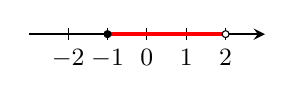
\begin{tikzpicture}[scale=0.5, font=\small]
  % Drawing the real number line
  \draw[thick, -stealth] (-3,0) -- (3,0); % Main line with arrow
  \foreach \x in {-2,-1,0,1,2} {
    \draw (\x,0.15) -- (\x,-0.15) node[below] {$\x$}; % Tick marks and labels
  }
  % \draw (0,0.3) -- (0,-0.3) node[below] {$0$}; % Emphasize origin

  % Marking the interval [-2, 3)
  \draw[line width=1.5pt, red] (-1,0) -- (2,0); % Thick line for interval
  \filldraw[black] (-1,0) circle (2.5pt); % Closed endpoint at -2
  \draw[black, fill=white] (2,0) circle (2.5pt); % Open endpoint at 3
\end{tikzpicture}
\\

\end{tabularx}
%ankicard end
